\documentclass[pdflatex,compress,mathserif]{beamer}

%\usetheme[dark,framenumber,totalframenumber]{ElektroITK}
\usetheme[darktitle,framenumber,totalframenumber]{ElektroITK}

\usepackage[utf8]{inputenc}
\usepackage[T1]{fontenc}
\usepackage{lmodern}
\usepackage[bahasai]{babel}
\usepackage{amsmath}
\usepackage{amsfonts}
\usepackage{amssymb}
\usepackage{graphicx}
\usepackage{multicol}
\usepackage{lipsum}

\newcommand*{\Scale}[2][4]{\scalebox{#1}{$#2$}}%

\title{PEMODELAN JARINGAN KOMUNIKASI}
\subtitle{Cisco Device Management}

\author{Tim Dosen Pengampu}

\begin{document}

\maketitle

\section{The Boot-up Process}

\begin{frame}
	\frametitle{Cisco Device Memory}
	\begin{itemize}
		\item Cisco routers and switches have 4 built-in memory locations:
		\begin{itemize}
			\item ROM – Read Only Memory
			\item Flash – newer devices use removable CompactFlash
			\item NVRAM – Non-Volatile RAM
			\item RAM – Random Access Memory
			\item An external USB device can also be used
		\end{itemize}
	\end{itemize}
\end{frame}

\begin{frame}
	\frametitle{ROM Read Only Memory}
	\begin{itemize}
		\item When the device is powered on, it will first load from ROM
		\item Two main functions are performed:
		\begin{enumerate}
			\item Power On Self Test (POST)
			\item Load bootstrap
		\end{enumerate}
		\item The bootstrap will look in Flash for an IOS software image to load
	\end{itemize}
\end{frame}

\begin{frame}{ROM Read Only Memory}
	\begin{itemize}
		\item If an IOS image cannot be found the device will show the ROMMON prompt at the command line
		\item The ROM Monitor can be used to recover a missing or corrupted software image
		\item In this case you can boot from USB or an external TFTP (Trivial File Transfer Protocol) server
		\item Search for ‘Cisco ROMMON Recovery’ for your device model
	\end{itemize}
\end{frame}

\begin{frame}
	\frametitle{Flash Memory}
	\begin{itemize}
		\item The system will load the first IOS image found in Flash by default
		\item You can override this with the boot system command
		\item You can copy additional IOS system images to Flash via TFTP or USB
	\end{itemize}
\end{frame}

\begin{frame}
	\frametitle{NVRAM Non-Volatile RAM Memory}
	\begin{itemize}
		\item When the system has finished loading the IOS system image from Flash, it will load the startup-config configuration file from NVRAM
		\item The saved startup-config becomes the current running-config in RAM
		\item If no startup-config file is found, the device will load the Setup Wizard
	\end{itemize}
\end{frame}

\begin{frame}{NVRAM Non-Volatile RAM Memory}
	\begin{itemize}
		\item Whenever you enter a command in IOS it takes effect immediately and goes into the running-config
		\item To make your changes permanent across a reboot:
		\item[] \texttt{copy running-config startup-config}
	\end{itemize}
\end{frame}

\begin{frame}
	\frametitle{RAM Random Access Memory}
	\begin{itemize}
		\item The IOS system image and startup-config are loaded from Flash and NVRAM into RAM during bootup
		\item RAM is used as the normal working memory of the device
		\item ROM, Flash and NVRAM are permanent memory, their contents are not lost when the device is powered off or rebooted
		\item RAM is volatile memory, its contents are lost when the device is powered off
	\end{itemize}
\end{frame}

\begin{frame}
	\frametitle{The VLAN Database}
	\begin{itemize}
		\item On a switch, the VLAN database (vlan.dat) is saved in either Flash or NVRAM, depending on the model of switch
	\end{itemize}
\end{frame}

\begin{frame}
	\frametitle{Booting from TFTP}
	\begin{itemize}
		\item The system can also load a system image and/or startup-config from an external TFTP server instead of Flash/NVRAM
		\item This is not recommended because the device will not be able to boot if it loses connectivity to the server. It is usually only used where the device does not have enough capacity in Flash to save the system image
	\end{itemize}
\end{frame}

\begin{frame}
	\frametitle{Lab Example}
	\begin{center}
		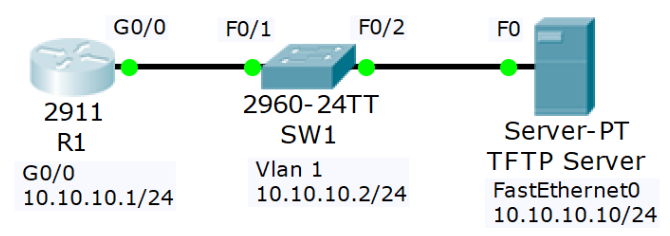
\includegraphics[width=0.7\linewidth]{img/img01}
	\end{center}
\end{frame}

\section{Factory Reset and Password Recovery}

\begin{frame}
	\frametitle{Factory Reset}
	\begin{itemize}
		\item To factory reset a router or switch:
		\item[] \texttt{write erase}
		\item This will erase the startup-config
		\item Reload to boot up with a blank configuration
		\item The Setup Wizard will run
	\end{itemize}
\end{frame}

\begin{frame}
	\frametitle{The Config Register}
	\begin{itemize}
		\item The configuration register can be used to change the way the router boots
		\item Use the \texttt{config-register} command in global configuration mode or \texttt{confreg} at the rommon prompt
		\item Eg \texttt{config-register 0x2142}
		\item[]
		\item 0x2102: boot normally (default)
		\item 0x2120: boot into rommon
		\item 0x2142: ignore contents of NVRAM (startup-config)
	\end{itemize}
\end{frame}

\begin{frame}
	\frametitle{Router Password Recovery Procedure}
	\begin{itemize}
		\item Press the break sequence (Ctrl-Break) at power on to break into rommon prompt
		\item \texttt{confreg 0x2142} to ignore the startup-config on boot
		\item The startup-config is still there with the full configuration including the unknown enable secret, but the router does not use it when it boots
		\item \texttt{reset} to reload
		\item The router will bootup with no configuration. Type \texttt{no} to bypass the setup wizard
		\item Enter enable mode. You will not be prompted for the enable secret as it is not in the running configuration
	\end{itemize}
\end{frame}

\begin{frame}{Router Password Recovery Procedure}
	\begin{itemize}
		\item Copy the startup config to the running config
		\item This will copy the entire previous configuration into the running config including the unknown enable secret. You are already in enable mode so you do not need to know what it is.
		\item Enter a new \texttt{enable secret} in global configuration mode to overwrite the old one. This will go into the running config
		\item \texttt{config-register 0x2102} so the router will boot normally on the next restart
		\item \texttt{copy run start} to save the configuration. This will merge the new enable password into the existing startup-config
	\end{itemize}
\end{frame}

\begin{frame}
	\frametitle{Switch Password Recovery Procedure}
	\begin{itemize}
		\item The switch password recovery procedure is very similar, but you may have to physically press the 'Mode' button on the front of the switch to break into the switch loader
		\item Search for 'Cisco password recovery' for your model of switch for full instructions
	\end{itemize}
\end{frame}

\section{Backing up the System Image and Configuration}

\begin{frame}
	\frametitle{Backing up the System Image\\and Config}
	\begin{itemize}
		\item Copies of the device’s IOS system image and configuration can be saved to Flash, FTP, TFTP or USB
		\item If you copy a config file into the running-config, it will be merged with the current configuration
		\item To replace a configuration, factory reset and then copy the new configuration into the startup-config
	\end{itemize}
	\texttt{copy flash tftp\\
		copy running-config tftp\\
		copy startup-config usb}
\end{frame}

\begin{frame}
	\frametitle{Lab Example}
	\begin{center}
		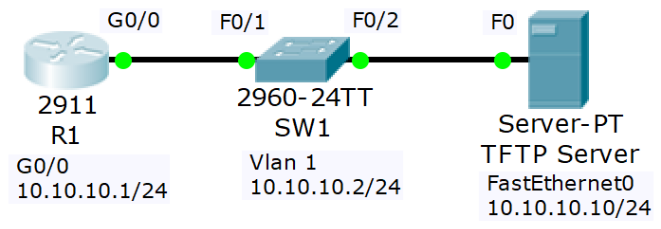
\includegraphics[width=0.7\linewidth]{img/img02}
	\end{center}
\end{frame}

\section{Upgrading IOS}

\begin{frame}
	\frametitle{Upgrading the IOS System Image}
	\begin{itemize}
		\item IOS software images can be downloaded from: \hyperlink{https://software.cisco.com/}{https://software.cisco.com/}
		\item After downloading the software, copy to the device’s Flash using TFTP: \texttt{copy tftp flash}
		\item Delete the old system image or use the \texttt{boot system} command
	\end{itemize}
\end{frame}

\begin{frame}
	\frametitle{Lab Example}
	\begin{center}
		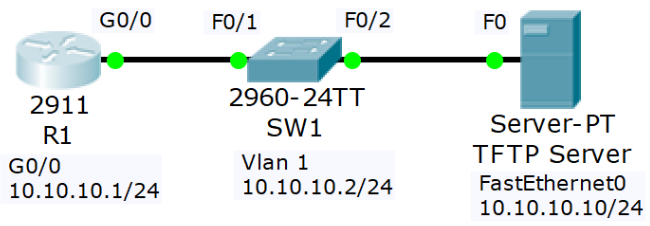
\includegraphics[width=0.7\linewidth]{img/img03}
	\end{center}
\end{frame}

\section{Licensing}

\begin{frame}
	\frametitle{Router IOS Licensing}
	\begin{itemize}
		\item Prior to IOS 15.0, different IOS system images were available for different feature sets, such as Security or Telephony
		\item Licensing was not enforced
		\item A universal system image is provided from IOS 15.0
		\item License codes must be entered to activate the Technology Packages
	\end{itemize}
\end{frame}

\begin{frame}
	\frametitle{Licensing Procedure}
	\begin{itemize}
		\item When you purchase a license you will be provided with a Product Activation Key (PAK) code
		\item The license will be tied to an individual device. To get the device's Unique Device Identifier (UDI) enter show license udi
		\item Go the the Cisco License Portal \hyperlink{http://www.cisco.com/go/license}{http://www.cisco.com/go/license} and enter the PAK code and UDI to generate the license
		\item Copy the license to Flash on the router
		\item \texttt{license install flash}:
		\item \texttt{license show}
	\end{itemize}
\end{frame}

\end{document}
